\chapter{Evaluation}
\label{cha:evaluation}
\section{Security}
\subsection{Automatic Vulnerability Scanners Testing}
Automatic web application vulnerability and penetration testing software was used to test security of the application. The following results were obtained: 
\begin{itemize}
    \item Wapiti (Open-source, ): \ref{fig:wapiti} (note: screenshot is trimmed, the rest of the report showed 0 vulnerabilities)
    \item ZAP (Open-source, made by OWASP): \ref{fig:zap}
    \item Intruder (Commercial, Large-scale grade): \ref{fig:intruder}
\end{itemize}
\begin{figure}
    
    \centering
    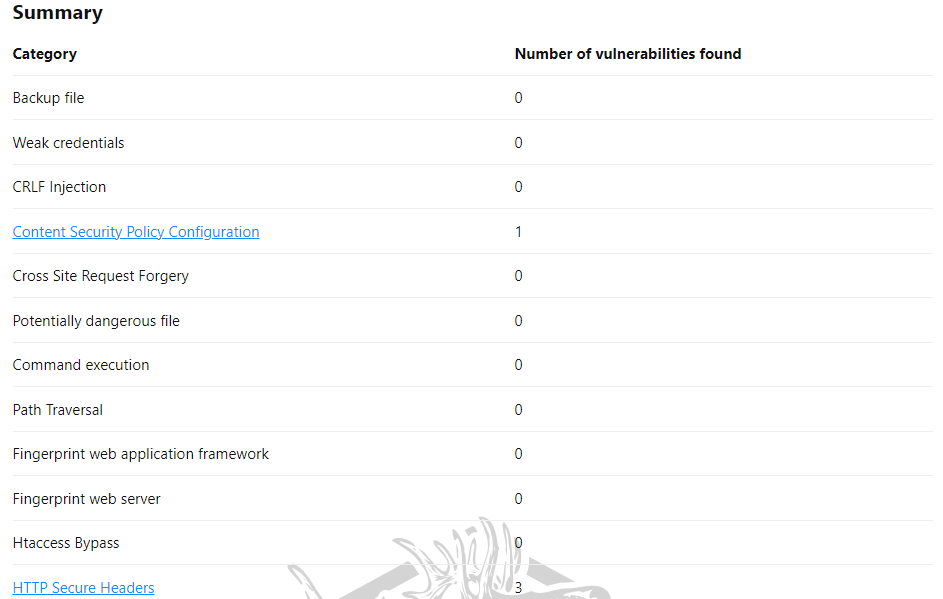
\includegraphics[width=0.9\textwidth,keepaspectratio]{../images/Wapiti.png}
    \caption{Wapiti scan result}
    \label{fig:wapiti}
    
\end{figure}
\begin{figure}
    
    \centering
    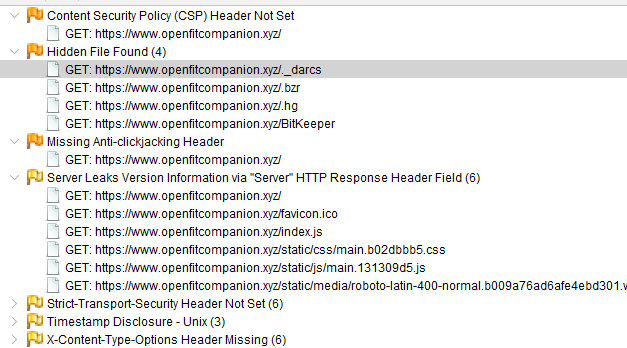
\includegraphics[width=0.8\textwidth,keepaspectratio]{../images/ZapResults.png}
    \caption{ZAP scan result}
    \label{fig:zap}
    
\end{figure}
\begin{figure}
    
    \centering
    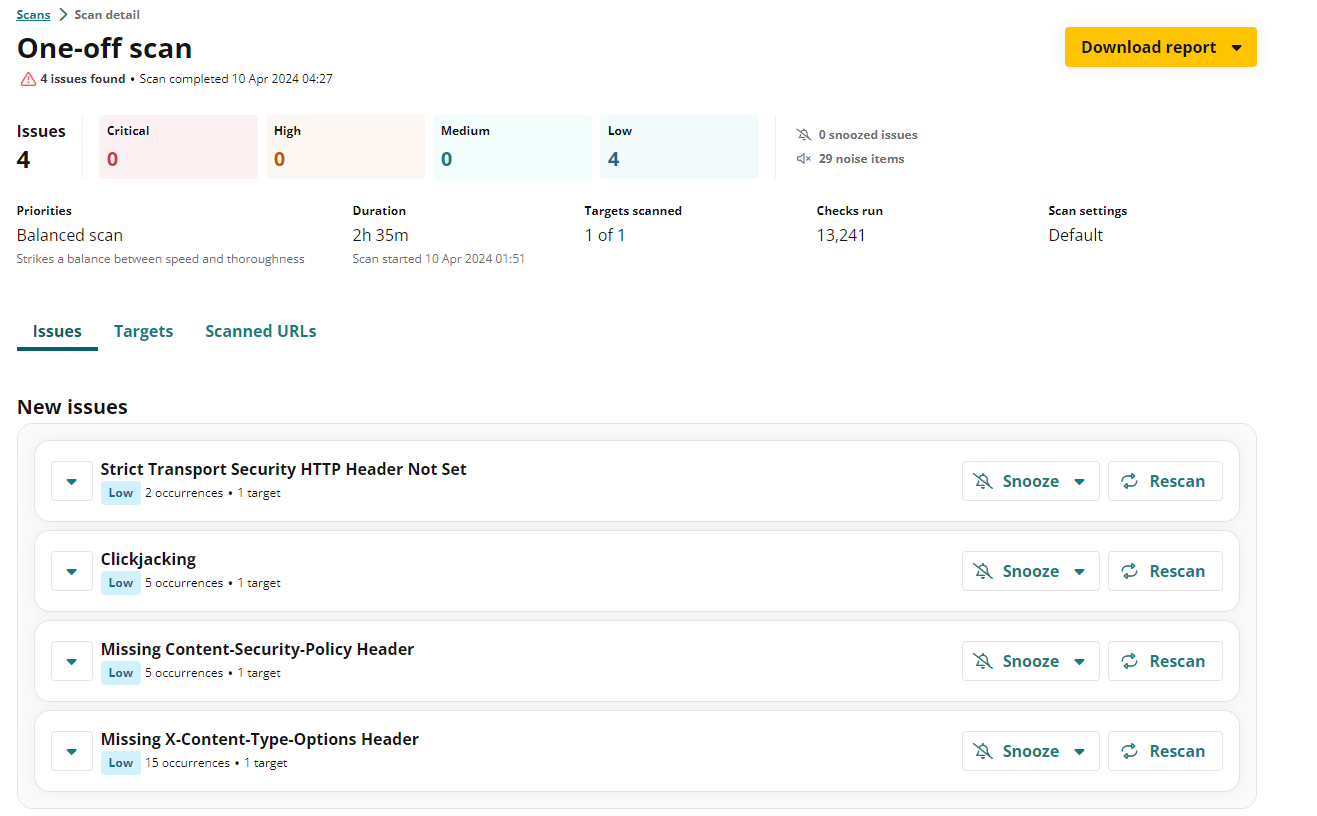
\includegraphics[width=1\textwidth,keepaspectratio]{../images/IntruderResults.png}
    \caption{Intruder scan result}
    \label{fig:intruder}
    
\end{figure}
\subsection{IAM}
\section{Cost}
\section{Function}
\section{Frontend Performance \& Accessibility \& UI}
\section{AI Insights Quality}
\section{Analysis results}
TODO: Do this chapter
